Di seguito verrà mostrato il lavoro svolto in collaborazione per avviare il progetto e, successivamente, verrà proposto ciascun contributo individuale apportato al progetto.

Nello specifico il lavoro inizialmente si è concentrato sullo studio, lo sviluppo e la scrittura di Smart Contracts per i \textit{Non-Fungible token}. Tuttavia al termine dello sviluppo e dopo un attenta ricerca si è deciso di intraprendere una strada differente e di allinearsi alla proposta di Flow, per cui determinati contratti fondamentali vengono forniti come standard in cui sono definite funzioni e risorse necessarie per lo sviluppo di sistemi basati su questo tipo di elementi. 

Di conseguenza lo \textbf{standard NFT} è stato studiato e implementato in collaborazione e verrà analizzato nella sezione \ref{sez:Flow NFT standard}, mentre quello relativo ai \textit{FungibleToken} è stato studiato e integrato al progetto per poter essere utilizzato come strumento di utilità per permettere la vendita di NFT in cambio di criptovaluta; sono state integrate anche transazioni e scripts utili per effettuare il corretto \textit{setup} dell'ambiente di test e l'implementazione \textit{FlowToken} fornita dallo standard \cite{web:FT-Standard}.

Di seguito viene mostrata una versione semplificata dell'architettura del sistema in cui si evidenziano i principali componenti utilizzati e realizzati, e le interazioni con la rete. 

\begin{figure}[H]
    \centering
    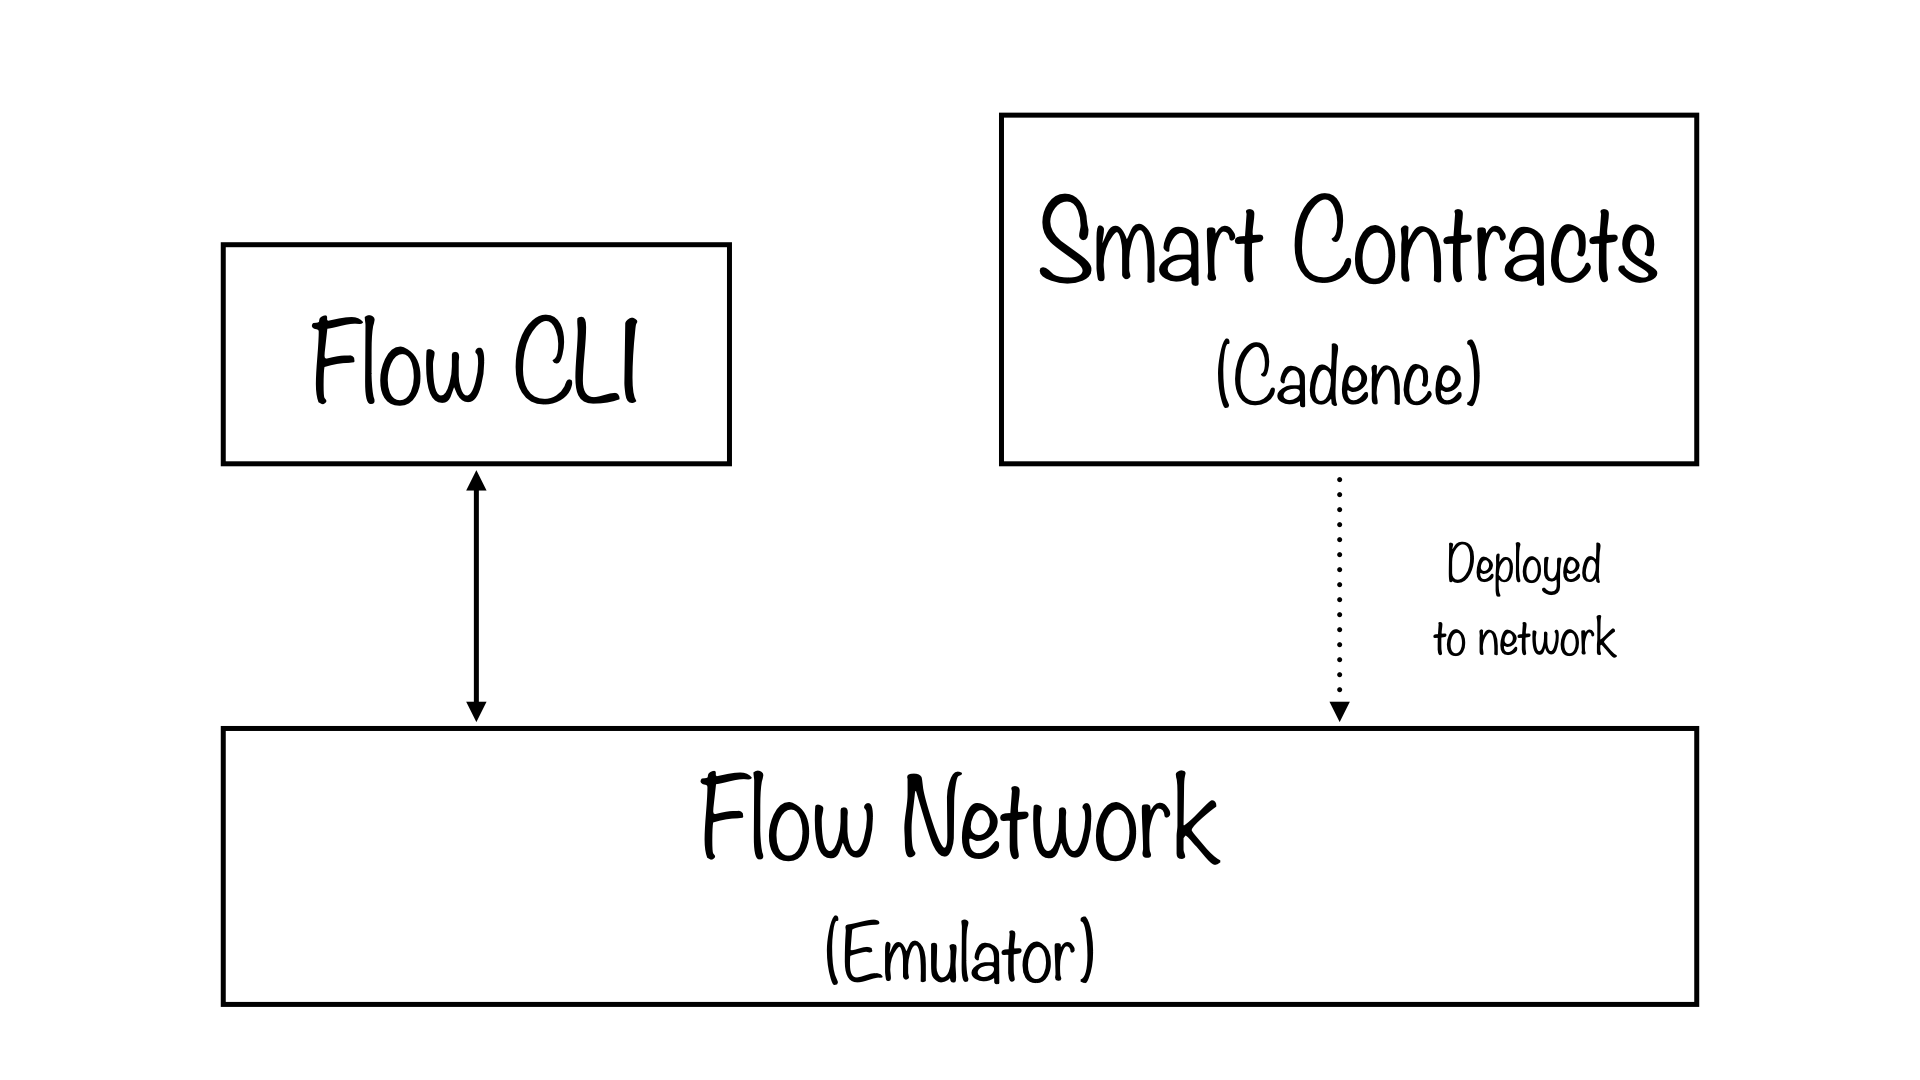
\includegraphics[width=0.8\textwidth]{img/ArchitetturaFlow.png}
    \caption{Architettura del sistema utilizzato}
    \label{fig:flowArch}
\end{figure}

Inoltre per semplificare la configurazione delle app, mette a disposizione un file chiamato \codeinline{flow.json} dal quale la CLI attinge alcune informazioni relative sia al deploy di contratti che ad indirizzi, chiavi pubbliche e aliases di determinati account, configurabili per ciascuna delle tre reti messe a disposizione da flow.

Workflow comune in use case standard (con certe ipotesi e.g. deployati certi contratti ecc...):

\begin{enumerate}
    \item Si apre il terminale
    \item Viene lanciato il flow emulator e si crea uno snapshot del DB per mantenerne le informazioni ai successivi avvii dell'emulatore
    \item Apro una nuova finestra del terminale (per Flow CLI)
    \item Setup degli account (emulatore, Alice e Bob)
    \begin{enumerate}
        \item Ogni account ha un tot di FT
        \item Crea una collezione per NFT e una capability 
        \item Creo risorsa Valut (deposito per FT)
        \item Creo capability per accedere al valut dell'account
    \end{enumerate}
    \item Minting di due NFT dall'emulatore 
    \item Trasferimento degli NFT mintati agli account Alice e Bob
\end{enumerate}

% \begin{lstlisting}[style=all, style=bash]
% # 1) Apro il terminale
% # 2) Viene lanciato il flow emulator (con snapshot del DB per mantenerne le informazioni ai successivi avvii dell'emulatore)
% # 3) Apro una nuova finestra del terminale (per Flow CLI)
% # 4) Setup degli account e minting dei FT (trasferiti agli account Alice e Bob) 
% \end{lstlisting}

\sezione{Flow NFT standard}{capitoli/implementazioni/NFT-Standard}

\sezione{Gallo}{capitoli/implementazioni/gallo}

\sezione{Gatto}{capitoli/implementazioni/gatto}

\sezione{Moli}{capitoli/implementazioni/moli}

\sezione{Problemi riscontrati}{capitoli/implementazioni/problemi}